\documentclass{article}\usepackage[]{graphicx}\usepackage[]{color}
%% maxwidth is the original width if it is less than linewidth
%% otherwise use linewidth (to make sure the graphics do not exceed the margin)
\makeatletter
\def\maxwidth{ %
  \ifdim\Gin@nat@width>\linewidth
    \linewidth
  \else
    \Gin@nat@width
  \fi
}
\makeatother

\definecolor{fgcolor}{rgb}{0.345, 0.345, 0.345}
\newcommand{\hlnum}[1]{\textcolor[rgb]{0.686,0.059,0.569}{#1}}%
\newcommand{\hlstr}[1]{\textcolor[rgb]{0.192,0.494,0.8}{#1}}%
\newcommand{\hlcom}[1]{\textcolor[rgb]{0.678,0.584,0.686}{\textit{#1}}}%
\newcommand{\hlopt}[1]{\textcolor[rgb]{0,0,0}{#1}}%
\newcommand{\hlstd}[1]{\textcolor[rgb]{0.345,0.345,0.345}{#1}}%
\newcommand{\hlkwa}[1]{\textcolor[rgb]{0.161,0.373,0.58}{\textbf{#1}}}%
\newcommand{\hlkwb}[1]{\textcolor[rgb]{0.69,0.353,0.396}{#1}}%
\newcommand{\hlkwc}[1]{\textcolor[rgb]{0.333,0.667,0.333}{#1}}%
\newcommand{\hlkwd}[1]{\textcolor[rgb]{0.737,0.353,0.396}{\textbf{#1}}}%
\let\hlipl\hlkwb

\usepackage{framed}
\makeatletter
\newenvironment{kframe}{%
 \def\at@end@of@kframe{}%
 \ifinner\ifhmode%
  \def\at@end@of@kframe{\end{minipage}}%
  \begin{minipage}{\columnwidth}%
 \fi\fi%
 \def\FrameCommand##1{\hskip\@totalleftmargin \hskip-\fboxsep
 \colorbox{shadecolor}{##1}\hskip-\fboxsep
     % There is no \\@totalrightmargin, so:
     \hskip-\linewidth \hskip-\@totalleftmargin \hskip\columnwidth}%
 \MakeFramed {\advance\hsize-\width
   \@totalleftmargin\z@ \linewidth\hsize
   \@setminipage}}%
 {\par\unskip\endMakeFramed%
 \at@end@of@kframe}
\makeatother

\definecolor{shadecolor}{rgb}{.97, .97, .97}
\definecolor{messagecolor}{rgb}{0, 0, 0}
\definecolor{warningcolor}{rgb}{1, 0, 1}
\definecolor{errorcolor}{rgb}{1, 0, 0}
\newenvironment{knitrout}{}{} % an empty environment to be redefined in TeX

\usepackage{alltt}

\usepackage{fancyhdr} % Required for custom headers
\usepackage{lastpage} % Required to determine the last page for the footer
\usepackage{extramarks} % Required for headers and footers
\usepackage{graphicx} % Required to insert images
\usepackage{hyperref}
\usepackage{amsmath} %for binomial pdf
\usepackage{parskip} % so that there's space bw paragraphs
\usepackage{float}
\usepackage{amsfonts}
\usepackage{verbatim}
\usepackage{undertilde}
\graphicspath{"~/almhub_0823/exp_design"}



% Margins
\topmargin=-0.45in
\evensidemargin=0in
\oddsidemargin=0in
\textwidth=6.5in
\textheight=9.0in
\headsep=0.25in 

\linespread{1.1} % Line spacing

% Set up the header and footer
\pagestyle{fancy}
\lhead{STAT 541: Experimental Design} % Top left header
\chead{Take Home Mid-term Corrections} % Top center header
\rhead{Andrea Mack} % Top right header
\lfoot{03/20/2017} % Bottom left footer
\cfoot{} % Bottom center footer
\rfoot{Page\ \thepage\ of\ \pageref{LastPage}} % Bottom right footer
\renewcommand\headrulewidth{0.4pt} % Size of the header rule
\renewcommand\footrulewidth{0.4pt} % Size of the footer rule

\setlength\parindent{0pt} % Removes all indentation from paragraphs
\setlength\parskip{0.5cm}
\restylefloat{table}

%----------------------------------------------------------------------------------------
%	DOCUMENT STRUCTURE COMMANDS
%	Skip this unless you know what you're doing
%----------------------------------------------------------------------------------------

% Header and footer for when a page split occurs within a problem environment
\newcommand{\enterProblemHeader}[1]{
\nobreak\extramarks{#1}{#1 continued on next page\ldots}\nobreak
\nobreak\extramarks{#1 (continued)}{#1 continued on next page\ldots}\nobreak
}

% Header and footer for when a page split occurs between problem environments
\newcommand{\exitProblemHeader}[1]{
\nobreak\extramarks{#1 (continued)}{#1 continued on next page\ldots}\nobreak
\nobreak\extramarks{#1}{}\nobreak
}


%----------------------------------------------------------------------------------------%
\IfFileExists{upquote.sty}{\usepackage{upquote}}{}
\begin{document}



\begin{enumerate}
\setcounter{enumi}{3}
\item {\it Use the sample means and an estimate of $\sigma$ based on the oneway ANOVA to estimate the sample size needed for a CRD to achieve:}

\begin{knitrout}\footnotesize
\definecolor{shadecolor}{rgb}{0.969, 0.969, 0.969}\color{fgcolor}\begin{kframe}
\begin{alltt}
\hlcom{# create dataset with means}
\hlstd{nitrogen} \hlkwb{<-} \hlkwd{c}\hlstd{(}\hlkwd{rep}\hlstd{(}\hlnum{1}\hlstd{,}\hlnum{4}\hlstd{),} \hlkwd{rep}\hlstd{(}\hlnum{2}\hlstd{,}\hlnum{4}\hlstd{),} \hlkwd{rep}\hlstd{(}\hlnum{3}\hlstd{,}\hlnum{4}\hlstd{),} \hlkwd{rep}\hlstd{(}\hlnum{4}\hlstd{,}\hlnum{4}\hlstd{),} \hlkwd{rep}\hlstd{(}\hlnum{5}\hlstd{,}\hlnum{4}\hlstd{),} \hlkwd{rep}\hlstd{(}\hlnum{6}\hlstd{,}\hlnum{4}\hlstd{))}
\hlstd{reps} \hlkwb{<-} \hlkwd{c}\hlstd{(}\hlkwd{rep}\hlstd{(}\hlkwd{c}\hlstd{(}\hlnum{1}\hlstd{,}\hlnum{2}\hlstd{,}\hlnum{3}\hlstd{,}\hlnum{4}\hlstd{),} \hlnum{6}\hlstd{))}
\hlstd{yield} \hlkwb{<-} \hlkwd{c}\hlstd{(}\hlnum{32.1}\hlstd{,}\hlnum{35.6}\hlstd{,}\hlnum{41.9}\hlstd{,}\hlnum{35.4}\hlstd{,}\hlnum{30.1}\hlstd{,}\hlnum{31.5}\hlstd{,}\hlnum{37.1}\hlstd{,}\hlnum{30.8}\hlstd{,}
           \hlnum{25.4}\hlstd{,}\hlnum{27.4}\hlstd{,}\hlnum{33.8}\hlstd{,}\hlnum{31.1}\hlstd{,}\hlnum{24.1}\hlstd{,}\hlnum{33.0}\hlstd{,}\hlnum{35.6}\hlstd{,}\hlnum{31.4}\hlstd{,}
           \hlnum{26.1}\hlstd{,}\hlnum{31}\hlstd{,}\hlnum{33.8}\hlstd{,}\hlnum{31.9}\hlstd{,}\hlnum{23.2}\hlstd{,}\hlnum{24.8}\hlstd{,}\hlnum{26.7}\hlstd{,}\hlnum{26.7}\hlstd{)}

\hlstd{p4} \hlkwb{<-} \hlkwd{data.frame}\hlstd{(}\hlkwd{cbind}\hlstd{(nitrogen, reps, yield))}
\hlstd{p4}\hlopt{$}\hlstd{nitrogen} \hlkwb{<-} \hlkwd{as.factor}\hlstd{(}\hlkwd{as.character}\hlstd{(p4}\hlopt{$}\hlstd{nitrogen))}

\hlstd{p4means} \hlkwb{<-} \hlkwd{aggregate}\hlstd{(p4}\hlopt{$}\hlstd{yield,} \hlkwd{list}\hlstd{(p4}\hlopt{$}\hlstd{nitrogen), mean)}
\hlkwd{colnames}\hlstd{(p4means)} \hlkwb{<-} \hlkwd{c}\hlstd{(}\hlstr{"Nitrogen"}\hlstd{,} \hlstr{"Mean"}\hlstd{)}

\hlcom{#write.csv(p4, file = "p4.csv")}
\hlcom{#write.csv(p4means, file = "p4means.csv")}
\hlcom{#check}
\hlstd{t1} \hlkwb{<-} \hlkwd{c}\hlstd{(}\hlnum{32.1}\hlstd{,}\hlnum{35.6}\hlstd{,}\hlnum{41.9}\hlstd{,}\hlnum{35.4}\hlstd{)}
\hlstd{t2} \hlkwb{<-} \hlkwd{c}\hlstd{(}\hlnum{30.1}\hlstd{,}\hlnum{31.5}\hlstd{,}\hlnum{37.1}\hlstd{,}\hlnum{30.8}\hlstd{)}
\hlstd{t3} \hlkwb{<-} \hlkwd{c}\hlstd{(}\hlnum{25.4}\hlstd{,}\hlnum{27.4}\hlstd{,}\hlnum{33.8}\hlstd{,}\hlnum{31.1}\hlstd{)}
\hlstd{t4} \hlkwb{<-} \hlkwd{c}\hlstd{(}\hlnum{24.1}\hlstd{,}\hlnum{33}\hlstd{,}\hlnum{35.6}\hlstd{,}\hlnum{31.4}\hlstd{)}
\hlstd{t5} \hlkwb{<-} \hlkwd{c}\hlstd{(}\hlnum{26.1}\hlstd{,}\hlnum{31}\hlstd{,}\hlnum{33.8}\hlstd{,}\hlnum{31.9}\hlstd{)}
\hlstd{t6} \hlkwb{<-} \hlkwd{c}\hlstd{(}\hlnum{23.2}\hlstd{,}\hlnum{24.8}\hlstd{,}\hlnum{26.7}\hlstd{,}\hlnum{26.7}\hlstd{)}

\hlkwd{apply}\hlstd{(}\hlkwd{data.frame}\hlstd{(}\hlkwd{cbind}\hlstd{(t1,t2,t3,t4,t5,t6)),} \hlnum{2}\hlstd{, mean)}
\end{alltt}
\begin{verbatim}
    t1     t2     t3     t4     t5     t6 
36.250 32.375 29.425 31.025 30.700 25.350 
\end{verbatim}
\end{kframe}
\end{knitrout}

\begin{verbatim}
proc glm data=p4meansdata;
class nitrogen;
model yield=nitrogen /ss3 solution;
run;
\end{verbatim}

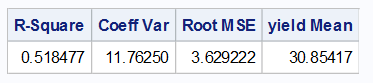
\includegraphics{prob4rmse}

\begin{verbatim}
PROC GLMPOWER DATA = p4means;
CLASS nitrogen;
MODEL mean=nitrogen;
POWER
STDDEV = 3.629222
ALPHA = 0.05 0.01
NTOTAL = .
POWER = 0.9 0.91 0.92 0.93 0.94 0.95;
RUN;
\end{verbatim}

\begin{center}
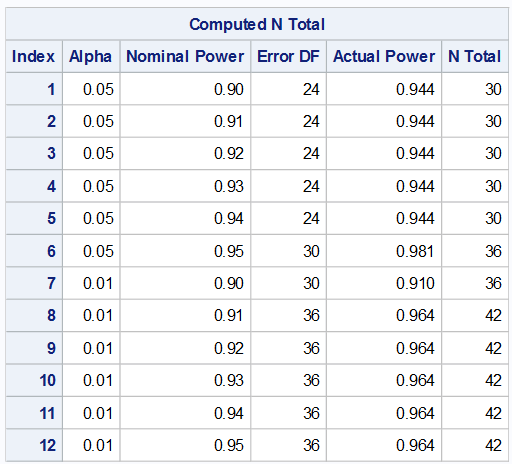
\includegraphics[scale=0.5]{prob4power}
\end{center}

\begin{enumerate}
\item {\it A power of at least 0.95 for the ANOVA F-test assuming $\alpha$ = 0.05.}

Using a total sample size of 36 (6 per group), the observed power is 0.979.

\item {\it A power of at least 0.90 for the ANOVA F-test assuming $\alpha$ = 0.01.}

Using a total sample size of 36 (6 per group), with these parameters set we get a power of 0.901.

\item {\it What would the estimated power for the ANOVA F-test assuming n=2 replicates are to be taken for each treatment and assuming $\alpha$ = 0.05?}
\end{enumerate}


The computed power is 0.324.

\begin{verbatim}
PROC GLMPOWER DATA = p4means;
CLASS nitrogen;
MODEL mean=nitrogen;
POWER
STDDEV = 3.629222
ALPHA = 0.05
NTOTAL = 12
POWER = .
;
RUN;
\end{verbatim}

\begin{center}
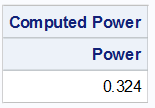
\includegraphics{prob42power}
\end{center}


\begin{center}
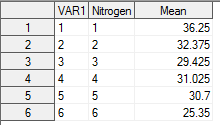
\includegraphics{prob4meandata}
\end{center}



\item %5
{\it  (5pt) Stat 541 Students: Read Section 4.3 (pages 165-168) on Graeco-Latin squares. Consider the
following experiment. A food processor wants to determine the effect of package design on the sale of
one of her company's products. She had five designs to be tested: A, B, C, D, E. There were several
sources of variation, however, whose possible effects were to be accounted for in the study. These
included (1) day of the week, (2) differences among stores, and (3) effect of shelf height. She decided
to use a Graeco-Latin square with five weekdays (M, Tu, W, Th, F,) for the row blocks, five stores
for the column blocks, and five shelf heights for the Greek letter blocks. The experimental design
and sales in dollars are shown in the following table.
}

In the original dataset, I had missed one column of the {\it latin} letters, making an incorrect dataset.

\begin{knitrout}\footnotesize
\definecolor{shadecolor}{rgb}{0.969, 0.969, 0.969}\color{fgcolor}\begin{kframe}
\begin{alltt}
\hlcom{# create latin squares data set}

\hlstd{rowsday} \hlkwb{<-} \hlkwd{c}\hlstd{(}\hlkwd{rep}\hlstd{(}\hlkwd{c}\hlstd{(}\hlstr{"Mon"}\hlstd{,} \hlstr{"Tues"}\hlstd{,} \hlstr{"Wed"}\hlstd{,} \hlstr{"Thurs"}\hlstd{,} \hlstr{"Fri"}\hlstd{),}\hlnum{5}\hlstd{))}
\hlstd{colstore} \hlkwb{<-} \hlkwd{c}\hlstd{(}\hlkwd{rep}\hlstd{(}\hlstr{"I"}\hlstd{,} \hlnum{5}\hlstd{),} \hlkwd{rep}\hlstd{(}\hlstr{"II"}\hlstd{,} \hlnum{5}\hlstd{),} \hlkwd{rep}\hlstd{(}\hlstr{"III"}\hlstd{,} \hlnum{5}\hlstd{),}
              \hlkwd{rep}\hlstd{(}\hlstr{"IV"}\hlstd{,} \hlnum{5}\hlstd{),} \hlkwd{rep}\hlstd{(}\hlstr{"V"}\hlstd{,} \hlnum{5}\hlstd{))}
\hlstd{latin} \hlkwb{<-} \hlkwd{c}\hlstd{(}\hlstr{"E"}\hlstd{,} \hlstr{"D"}\hlstd{,} \hlstr{"B"}\hlstd{,} \hlstr{"C"}\hlstd{,} \hlstr{"A"}\hlstd{,} \hlstr{"C"}\hlstd{,} \hlstr{"B"}\hlstd{,} \hlstr{"E"}\hlstd{,} \hlstr{"A"}\hlstd{,} \hlstr{"D"}\hlstd{,}
           \hlstr{"B"}\hlstd{,} \hlstr{"A"}\hlstd{,} \hlstr{"D"}\hlstd{,} \hlstr{"E"}\hlstd{,} \hlstr{"C"}\hlstd{,}\hlstr{"D"}\hlstd{,} \hlstr{"C"}\hlstd{,} \hlstr{"A"}\hlstd{,} \hlstr{"B"}\hlstd{,} \hlstr{"E"}\hlstd{,} \hlstr{"A"}\hlstd{,} \hlstr{"E"}\hlstd{,} \hlstr{"C"}\hlstd{,} \hlstr{"D"}\hlstd{,} \hlstr{"B"}\hlstd{)}

\hlstd{greek} \hlkwb{<-} \hlkwd{c}\hlstd{(}\hlstr{"alpha"}\hlstd{,} \hlstr{"delta"}\hlstd{,} \hlstr{"epsilon"}\hlstd{,} \hlstr{"beta"}\hlstd{,} \hlstr{"gamma"}\hlstd{,} \hlstr{"delta"}\hlstd{,}
           \hlstr{"beta"}\hlstd{,} \hlstr{"gamma"}\hlstd{,} \hlstr{"epsilon"}\hlstd{,} \hlstr{"alpha"}\hlstd{,} \hlstr{"gamma"}\hlstd{,} \hlstr{"alpha"}\hlstd{,}
           \hlstr{"beta"}\hlstd{,} \hlstr{"delta"}\hlstd{,} \hlstr{"epsilon"}\hlstd{,} \hlstr{"epsilon"}\hlstd{,} \hlstr{"gamma"}\hlstd{,} \hlstr{"delta"}\hlstd{,}
           \hlstr{"alpha"}\hlstd{,} \hlstr{"beta"}\hlstd{,} \hlstr{"beta"}\hlstd{,} \hlstr{"epsilon"}\hlstd{,} \hlstr{"alpha"}\hlstd{,} \hlstr{"gamma"}\hlstd{,} \hlstr{"delta"}\hlstd{)}

\hlstd{dollars} \hlkwb{<-} \hlkwd{c}\hlstd{(}\hlnum{238}\hlstd{,}\hlnum{149}\hlstd{,}\hlnum{222}\hlstd{,}\hlnum{187}\hlstd{,}\hlnum{65}\hlstd{,}\hlnum{228}\hlstd{,}\hlnum{220}\hlstd{,}\hlnum{295}\hlstd{,}\hlnum{66}\hlstd{,}\hlnum{118}\hlstd{,}\hlnum{158}\hlstd{,}\hlnum{92}\hlstd{,}\hlnum{104}\hlstd{,}\hlnum{242}\hlstd{,}
             \hlnum{279}\hlstd{,}\hlnum{188}\hlstd{,}\hlnum{169}\hlstd{,}\hlnum{54}\hlstd{,}\hlnum{122}\hlstd{,}\hlnum{278}\hlstd{,}\hlnum{74}\hlstd{,}\hlnum{282}\hlstd{,}\hlnum{213}\hlstd{,}\hlnum{90}\hlstd{,}\hlnum{176}\hlstd{)}

\hlstd{p5data} \hlkwb{<-} \hlkwd{data.frame}\hlstd{(}\hlkwd{cbind}\hlstd{(rowsday, colstore, latin, greek, dollars))}

\hlkwd{dim}\hlstd{(p5data)}
\end{alltt}
\begin{verbatim}
[1] 25  5
\end{verbatim}
\begin{alltt}
\hlkwd{aggregate}\hlstd{(}\hlkwd{as.numeric}\hlstd{(}\hlkwd{as.character}\hlstd{(p5data}\hlopt{$}\hlstd{dollars)),} \hlkwd{list}\hlstd{(}\hlkwd{as.factor}\hlstd{(p5data}\hlopt{$}\hlstd{rowsday)), mean)}
\end{alltt}
\begin{verbatim}
  Group.1     x
1     Fri 183.2
2     Mon 177.2
3   Thurs 141.4
4    Tues 182.4
5     Wed 177.6
\end{verbatim}
\begin{alltt}
\hlcom{#write.csv(p5data, file = "p5data.csv")}

\hlstd{mon} \hlkwb{<-} \hlkwd{c}\hlstd{(}\hlnum{238}\hlstd{,}\hlnum{228}\hlstd{,}\hlnum{158}\hlstd{,}\hlnum{188}\hlstd{,}\hlnum{74}\hlstd{)}
\hlstd{tues} \hlkwb{<-} \hlkwd{c}\hlstd{(}\hlnum{149}\hlstd{,}\hlnum{220}\hlstd{,}\hlnum{92}\hlstd{,}\hlnum{169}\hlstd{,}\hlnum{282}\hlstd{)}
\hlstd{wed} \hlkwb{<-} \hlkwd{c}\hlstd{(}\hlnum{222}\hlstd{,}\hlnum{295}\hlstd{,}\hlnum{104}\hlstd{,}\hlnum{54}\hlstd{,}\hlnum{213}\hlstd{)}
\hlstd{thurs} \hlkwb{<-} \hlkwd{c}\hlstd{(}\hlnum{187}\hlstd{,}\hlnum{66}\hlstd{,}\hlnum{242}\hlstd{,}\hlnum{122}\hlstd{,}\hlnum{90}\hlstd{)}
\hlstd{fri} \hlkwb{<-} \hlkwd{c}\hlstd{(}\hlnum{65}\hlstd{,}\hlnum{118}\hlstd{,}\hlnum{279}\hlstd{,}\hlnum{278}\hlstd{,}\hlnum{176}\hlstd{)}
\hlkwd{c}\hlstd{(}\hlkwd{mean}\hlstd{(mon),} \hlkwd{mean}\hlstd{(tues),} \hlkwd{mean}\hlstd{(wed),} \hlkwd{mean}\hlstd{(thurs),} \hlkwd{mean}\hlstd{(fri))}
\end{alltt}
\begin{verbatim}
[1] 177.2 182.4 177.6 141.4 183.2
\end{verbatim}
\end{kframe}
\end{knitrout}

\begin{enumerate}
\item
{\it Perform an ANOVA. State the null and alternative hypotheses of interest, and your conclusions.
You can use $\alpha$ = .05 for testing.}

$Y_{ijkl} = \mu + \beta_{i} + \gamma_{j} + \psi_{k} + \tau_{l} + \epsilon_{ijkl}$

Let $\tau_{l}$ represents the effect of design l which is an element of the set A,B,C,D,E.

$H_{o}$: $\tau_{A} = \tau_{B} = \tau_{C} = \tau_{D} = \tau_{E}$

$H_{a}$: at least one $\tau_{l} \neq \tau_{l'}$ for $l \neq l'$

There is strong evidence of a design effect on the true mean price (P\textless0.0001). At the $\alpha$ =  0.05 cutoff, the design did have an effect on the true mean price after accounting for the store, shelf, and weekday effects.

\begin{verbatim}
proc glm data=p5data1; 
title 'Graeco-Latin Square';
class rowsday colstore latin greek;
model newdollar = rowsday colstore latin greek;
means latin / tukey alpha=0.05;
run;
\end{verbatim}

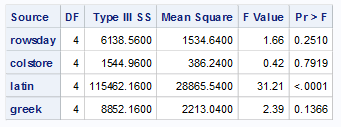
\includegraphics{latin1}


\item
{\it  Include a Tukey multiple comparison procedure, and your conclusions from it.}

The empirical mean cost increased in the order of A, D, B, C, and the highest mean cost was with design E. Using the 95\% Tukey adjusted family-wise confidence level, there is no evidence the mean cost differed for designs A and D, but strong evidence mean cost for design A  differed from mean cost for designs B, C, and E. There is no evidence the mean cost differed for designs D and B, but strong evidence mean cost for design D differed from mean cost from designs C and E. There is no evidence mean cost for design B differed from that of design C, but strong evidence mean cost for design B differed from mean cost of design E. There is no evidence mean cost of design C differed from mean cost of design E. 

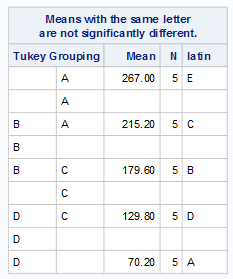
\includegraphics{latintuk1}

\end{enumerate}

\end{enumerate}
\end{document}
